\documentclass[border=3pt]{standalone}
\usepackage{fontspec}
\setmainfont{Times New Roman}
\usepackage{pgfplots}
\pgfplotsset{compat=1.18}
\usetikzlibrary{arrows.meta,calc,positioning,shapes.geometric}
\definecolor{forest}{HTML}{346E57}
\definecolor{sage}{HTML}{E8EFEA}
\definecolor{clay}{HTML}{B77E60}
\definecolor{gray}{HTML}{718078}
\definecolor{rule}{HTML}{B7C3BA}
\definecolor{ink}{HTML}{000000}
\begin{document}
\hyphenpenalty=10000\exhyphenpenalty=10000
\fontsize{10}{12}\selectfont
\renewcommand{\small}{\fontsize{9}{11}\selectfont}
\renewcommand{\scriptsize}{\fontsize{8}{10}\selectfont}
\resizebox{14cm}{!}{%
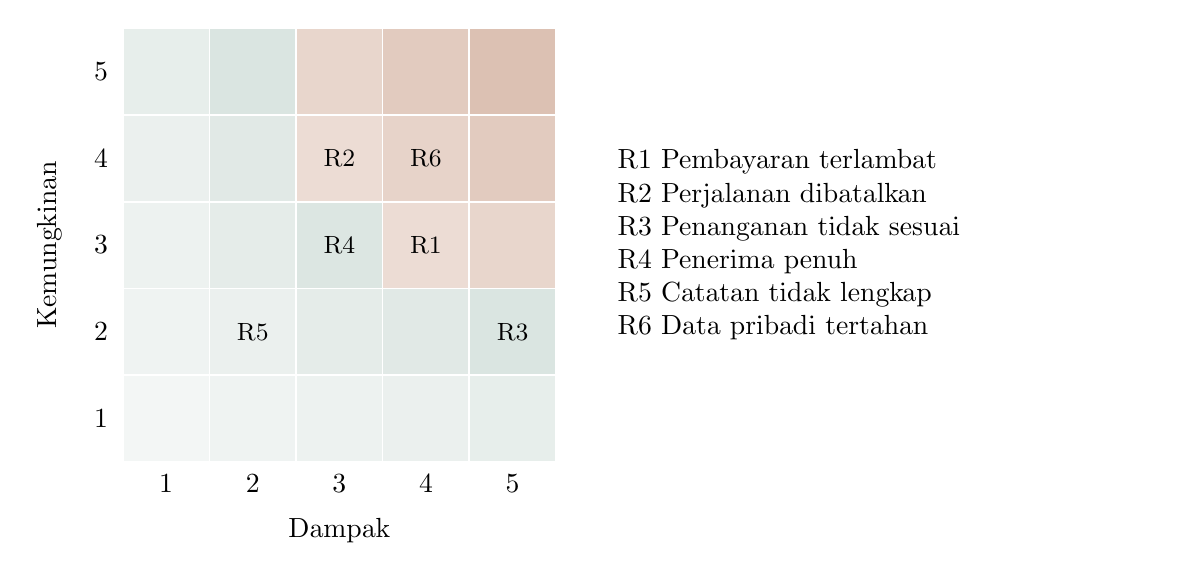
\begin{tikzpicture}[x=1.1cm,y=1.1cm]
\filldraw[fill=forest!6,draw=white,line width=.6pt] (0,0) rectangle (1,1);
\filldraw[fill=forest!8,draw=white,line width=.6pt] (1,0) rectangle (2,1);
\filldraw[fill=forest!9,draw=white,line width=.6pt] (2,0) rectangle (3,1);
\filldraw[fill=forest!10,draw=white,line width=.6pt] (3,0) rectangle (4,1);
\filldraw[fill=forest!12,draw=white,line width=.6pt] (4,0) rectangle (5,1);
\filldraw[fill=forest!8,draw=white,line width=.6pt] (0,1) rectangle (1,2);
\filldraw[fill=forest!10,draw=white,line width=.6pt] (1,1) rectangle (2,2);
\node[align=center,text width=.95cm,font=\small] at (1.5,1.5) {R5};
\filldraw[fill=forest!13,draw=white,line width=.6pt] (2,1) rectangle (3,2);
\filldraw[fill=forest!15,draw=white,line width=.6pt] (3,1) rectangle (4,2);
\filldraw[fill=forest!18,draw=white,line width=.6pt] (4,1) rectangle (5,2);
\node[align=center,text width=.95cm,font=\small] at (4.5,1.5) {R3};
\filldraw[fill=forest!9,draw=white,line width=.6pt] (0,2) rectangle (1,3);
\filldraw[fill=forest!13,draw=white,line width=.6pt] (1,2) rectangle (2,3);
\filldraw[fill=forest!17,draw=white,line width=.6pt] (2,2) rectangle (3,3);
\node[align=center,text width=.95cm,font=\small] at (2.5,2.5) {R4};
\filldraw[fill=clay!27,draw=white,line width=.6pt] (3,2) rectangle (4,3);
\node[align=center,text width=.95cm,font=\small] at (3.5,2.5) {R1};
\filldraw[fill=clay!32,draw=white,line width=.6pt] (4,2) rectangle (5,3);
\filldraw[fill=forest!10,draw=white,line width=.6pt] (0,3) rectangle (1,4);
\filldraw[fill=forest!15,draw=white,line width=.6pt] (1,3) rectangle (2,4);
\filldraw[fill=clay!27,draw=white,line width=.6pt] (2,3) rectangle (3,4);
\node[align=center,text width=.95cm,font=\small] at (2.5,3.5) {R2};
\filldraw[fill=clay!34,draw=white,line width=.6pt] (3,3) rectangle (4,4);
\node[align=center,text width=.95cm,font=\small] at (3.5,3.5) {R6};
\filldraw[fill=clay!40,draw=white,line width=.6pt] (4,3) rectangle (5,4);
\filldraw[fill=forest!12,draw=white,line width=.6pt] (0,4) rectangle (1,5);
\filldraw[fill=forest!18,draw=white,line width=.6pt] (1,4) rectangle (2,5);
\filldraw[fill=clay!32,draw=white,line width=.6pt] (2,4) rectangle (3,5);
\filldraw[fill=clay!40,draw=white,line width=.6pt] (3,4) rectangle (4,5);
\filldraw[fill=clay!48,draw=white,line width=.6pt] (4,4) rectangle (5,5);
\node at (0.5,-.25) {1};
\node at (-.25,0.5) {1};
\node at (1.5,-.25) {2};
\node at (-.25,1.5) {2};
\node at (2.5,-.25) {3};
\node at (-.25,2.5) {3};
\node at (3.5,-.25) {4};
\node at (-.25,3.5) {4};
\node at (4.5,-.25) {5};
\node at (-.25,4.5) {5};
\node at (2.5,-.8) {Dampak};
\node[rotate=90] at (-.85,2.5) {Kemungkinan};
\node[anchor=west,align=left,text width=6.8cm] at (5.6,2.5) {R1 Pembayaran terlambat\\R2 Perjalanan dibatalkan\\R3 Penanganan tidak sesuai\\R4 Penerima penuh\\R5 Catatan tidak lengkap\\R6 Data pribadi tertahan};
\end{tikzpicture}
}

\end{document}
